\documentclass{article}

\usepackage{amsmath}
\usepackage{amssymb}
\usepackage{graphicx}
\usepackage{fullpage}

\title{Reflection prediction}
\author{David Waterman}
\date{}

\begin{document}

\maketitle

\section*{Introduction}
This document contains the mathematical description of reflection prediction formulae and derivatives thereof with respect to some model parameters.
It is based on the LURE notes and Bricogne's 1987 CCP4 Proceedings on the EEC Cooperative Programming Workshop on Position-Sensitive
Detector Software. The purpose here is to put the notes in a concise form and in a single place.

\section*{Projection to the abstract detector plane}
\begin{center}
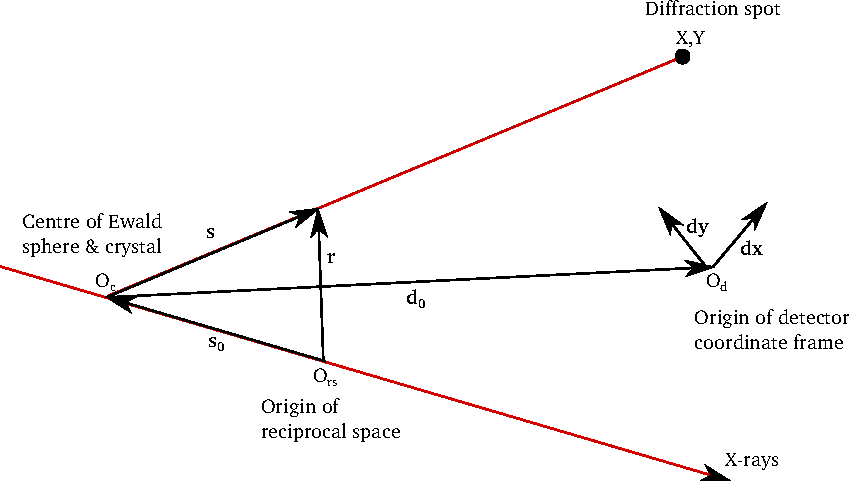
\includegraphics{diffraction_geometry.pdf}
\end{center}
The nomenclature used here follows my handwritten notes. We should update this document with our own conventions, where they differ.

$\vec{r}$ is the reciprocal lattice vector

$\vec{s} $ is the diffraction vector

$\vec{s_0}$ is the source vector (directed towards the source)

$\vec{d_0}$ is the detector frame origin vector

$\vec{d_x}$, $\vec{d_y}$ are the detector coordinate system basis vectors.


The projection from the Ewald sphere centre through the reciprocal lattice point (`relp') to the detector plane is
%
\begin{equation}
X \vec{d_x} + Y \vec{d_y} + \vec{d_0} = \alpha \vec{s}
\end{equation}

In matrix form,
\begin{equation}
\begin{pmatrix}
d_{x_1} &d_{y_1} &d_{0_1} \\
d_{x_2} &d_{y_2} &d_{0_2} \\
d_{x_3} &d_{y_3} &d_{0_3} \\
\end{pmatrix}
\begin{pmatrix}
X \\ Y \\ 1
\end{pmatrix} = \alpha \vec{s}
\end{equation}

Define matrices
\begin{equation}
\mathbf{d} = 
\begin{pmatrix}
d_{x_1} &d_{y_1} &d_{0_1} \\
d_{x_2} &d_{y_2} &d_{0_2} \\
d_{x_3} &d_{y_3} &d_{0_3} \\
\end{pmatrix} \textrm{ and }
\mathbf{D} = \mathbf{d}^{-1} = 
\begin{pmatrix}
\vec{D_x} | \vec{D_y} | \vec{D_0}
\end{pmatrix}^\mathrm{T}
\end{equation}

and a vector
\begin{equation}
\vec{v} = \begin{pmatrix}
u \\
v \\
w \\
\end{pmatrix} = \mathbf{D} \vec{s}
\end{equation}

then
\begin{equation}
\begin{pmatrix}
X \\ 
Y \\ 
1
\end{pmatrix} = \alpha \mathbf{D} \vec{s} = \alpha \vec{v} = \alpha
\begin{pmatrix}
u \\
v \\
w 
\end{pmatrix} 
\end{equation}

So $ X = \alpha u $, $ Y = \alpha v$, and $ w = \frac{1}{\alpha}$
\begin{equation}
X = \frac{u}{w} \textrm{ and } Y = \frac{v}{w}
\end{equation}

This means that $X$ and $Y$ can be obtained from calculation of $\mathbf{D}$ and knowledge of $\vec{s}$. The former
comes from the orientation of the detector plane and the latter is constructed as $\vec{s} = \vec{r} - \vec{s_0}$


\section*{Calculation of the rotation angle}

Diffraction occurs when $\vec{r_\phi}$ lies on the Ewald sphere, which is equivalent to
\begin{eqnarray}
\label{eq:diff_condit}
\vec{s} \cdot \vec{s} & = & \vec{s_0} \cdot \vec{s_0} \nonumber \\
\vec{r_\phi} \cdot \vec{r_\phi} - 2 \vec{r_\phi} \cdot \vec{s_0} - \vec{s_0} \cdot \vec{s_0} & = & \vec{s_0} \cdot \vec{s_0} \nonumber \\
\vec{r_\phi} \cdot \vec{r_\phi} - 2 \vec{r_\phi} \cdot \vec{s_0} & = & 0
\end{eqnarray}

Define $\vec{r_0}$ as $\vec{r_\phi}$ at $\phi = 0$

Now using Rodrigues' rotation formula

\begin{eqnarray}
\label{eq:rodrigues}
\vec{r_\phi} & = & \operatorname{R}(\vec{e}, \phi) \vec{r_0} \nonumber \\
 & = & \left( \vec{r_0} \cdot \vec{e} \right) \vec{e} + 
       \left( \vec{r_0} - \left( \vec{r_0} \cdot \vec{e} \right) \vec{e} \right) cos{\phi} +
       \left( \vec{e} \times \vec{r_0} \right) sin{\phi}
\end{eqnarray}

where $\vec{e}$ is the spindle axis.

Also we have $\vec{r_\phi} \cdot \vec{r_\phi} = \vec{r_0} \cdot \vec{r_0}$, which we substitute into Equation~\ref{eq:diff_condit} to give

\begin{equation}
\vec{r_0} \cdot \vec{r_0} - 2 \vec{r_\phi} \cdot \vec{s_0}  =  0
\end{equation}

Substitute for $\vec{r_\phi}$ from Equation~\ref{eq:rodrigues} and going through all the cancellations gives

\begin{equation}
\label{eq:prediction}
\left(
  \vec{r_0} \cdot \vec{s_0} - \left( \vec{r_0} \cdot \vec{e} \right) \left( \vec{e} \cdot \vec{s_0} \right)
\right) cos{\phi} + 
\vec{s_0} \cdot \left( \vec{e} \times \vec{r_0} \right) sin{\phi} = 
\frac{1}{2} \vec{r_0} \cdot \vec{r_0} - \left( \vec{r_0} \cdot \vec{e} \right) \left( \vec{e} \cdot \vec{s_0} \right)
\end{equation}

This is the prediction formula for rotation around a general spindle axis $\vec{e}$. As long as we know $\vec{s_0}$ and $\vec{e}$
from the experiment geometry, and we calculate $\vec{r_0}$ from the crystal setting matrix then Equation~\ref{eq:prediction} is of
the form $a cos{\phi} + b sin{\phi} = c$ with known $a$, $b$ and $c$.

\section*{Derivatives of the spot coordinates}
\end{document}
